\documentclass[aspectratio=169%可调屏宽比16:9(169),4:3(43)
,serif,mathserif]{beamer}
\mode<presentation>{
%\usetheme{default}
%\usetheme{AnnArbor}
%\usetheme{Antibes}
%\usetheme{Bergen}
%\usetheme{Berkeley}
%\usetheme{Berlin}
%\usetheme{Boadilla}
%\usetheme{CambridgeUS}
%\usetheme{Copenhagen}
%\usetheme{Darmstadt}
%\usetheme{Dresden}
%\usetheme{Frankfurt}
%\usetheme{Goettingen}
%\usetheme{Hannover}
%\usetheme{Ilmenau}
%\usetheme{JuanLesPins}
%\usetheme{Luebeck}
\usetheme{Madrid}
%\usetheme{Malmoe}
%\usetheme{Marburg}
%\usetheme{Montpellier}
%\usetheme{PaloAlto}
%\usetheme{Pittsburgh}
%\usetheme{Rochester}
%\usetheme{Singapore}
%\usetheme{Szeged}
%\usetheme{Warsaw}
% As well as themes, the Beamer class has a number of color themes
% for any slide theme. Uncomment each of these in turn to see how it
% changes the colors of your current slide theme.
%\usecolortheme{albatross}
%\usecolortheme{beaver}
%\usecolortheme{beetle}
%\usecolortheme{crane}
%\usecolortheme{dolphin}
%\usecolortheme{dove}
%\usecolortheme{fly}
%\usecolortheme{lily}
%\usecolortheme{orchid}
%\usecolortheme{rose}
%\usecolortheme{seagull}
%\usecolortheme{seahorse}
%\usecolortheme{whale}
%\usecolortheme{wolverine}
%\setbeamertemplate{footline} % To remove the footer line in all slides uncomment this line
%\setbeamertemplate{footline}[page number] % To replace the footer line in all slides with a simple slide count uncomment this line
%\setbeamertemplate{navigation symbols}{} % To remove the navigation symbols from the bottom of all slides uncomment this line
}
\usepackage{adjustbox}
\usepackage{indentfirst} 
\usepackage{amsmath, amsfonts, epsfig, xspace}
\usepackage{algorithm,algorithmic}
\usepackage{beamerthemesplit}
\usepackage{booktabs}
\usepackage{bm}
\usepackage{braket}
\usepackage{calligra}
\usepackage[T1]{fontenc}
\usepackage{fontspec}
\usepackage{ctex}
\usepackage{latexsym}
\usepackage{multicol}
\usepackage{multimedia}
\usepackage{calligra} \DeclareMathAlphabet{\mathcalligra}{T1}{calligra}{m}{n} \DeclareFontShape{T1}{calligra}{m}{n}{<->s*[2.2]callig15}{}
\usepackage{pstricks,pst-node}
\usepackage{ragged2e}
\usepackage{setspace}
\usepackage[normal,tight,center]{subfigure}
\setlength{\subfigcapskip}{-.5em}
\setlength{\parindent}{2em}
\begin{document}
\title[Integrating Simplex with DPLL(T)]{Integrating Simplex with DPLL(T)} % The short title appears at the bottom of every slide, the full title is only on the title page
\author[Chi~Zhiming]{迟智名} % Your name
\institute[LZU] % Your institution as it will appear on the bottom of every slide, may be shorthand to save space
{	
	%Lanzhou University \\ % Your institution for the title page
	%\medskip
	%\textit{chizhm16@lzu.edu.cn} % Your email address
}
	\CTEXoptions[today=old]
	\date{\today} % Date, can be changed to a custom date
\begin{frame}[plain]\vspace{1.5em}
\titlepage\vspace{-0.5cm}
%\centerline{\includegraphics[height=0.30\textheight]{logo.png}}
%\hfill 指导教师:焦桂梅
\end{frame}
\begin{frame}{目录}
\tableofcontents
\end{frame}
\AtBeginSection[]
{
\begin{frame}{\tiny}
\frametitle{目录}
\tableofcontents[currentsection]
\end{frame}
}
%----------------------------------------------------------------------------------------
%	PRESENTATION SLIDES
%----------------------------------------------------------------------------------------

%------------------------------------------------
\section{Contribution} % Sections can be created in order to organize your presentation into discrete blocks, all sections and subsections are automatically printed in the table of contents as an overview of the talk
%------------------------------------------------
%\subsection{Extract CFGs from RNN}
\begin{frame}
	\frametitle{Contribution}
\begin{itemize}		
	\item Prove a tight robustness guarantee in $L_2$ norm for randomized smoothing with Gaussian noise.
	\item We can have no knowledge about the base classifier beyond the distribution of $f(x+\epsilon)$
	\item The smoothed classifier is not itself a neural network, though it leverages the discriminative ability of a neural network base classifier. 
\end{itemize}
\end{frame}

\section{Randomized Smoothing}
\subsection{Introduction}
\begin{frame}
	\frametitle{Definition}
	\begin{definition}[Randomized Smoothing]
		Let $f: \mathbb{R}^d \to \mathcal{Y}$  be any deterministic or random function, and let 
		$ \varepsilon \sim  \mathcal{N}(0, \sigma^2 I)$ the smoothed classifier $g$ returns:
		\begin{equation}
			g(x)=\underset{c \in \mathcal{Y}}{\arg \max } \mathbb{P}(f(x+\varepsilon)=c)
		\end{equation}
	\end{definition}
	i.e.$g(x) = \underset{c \in \mathcal{Y}}{\arg \max}~m(c), m(c)= m(\{x^{\prime} \in \mathbb{R}^{d}: f(x^{\prime})=c\})$
\end{frame}

\begin{frame}
	\frametitle{Example}
	\begin{figure}[htbp]
		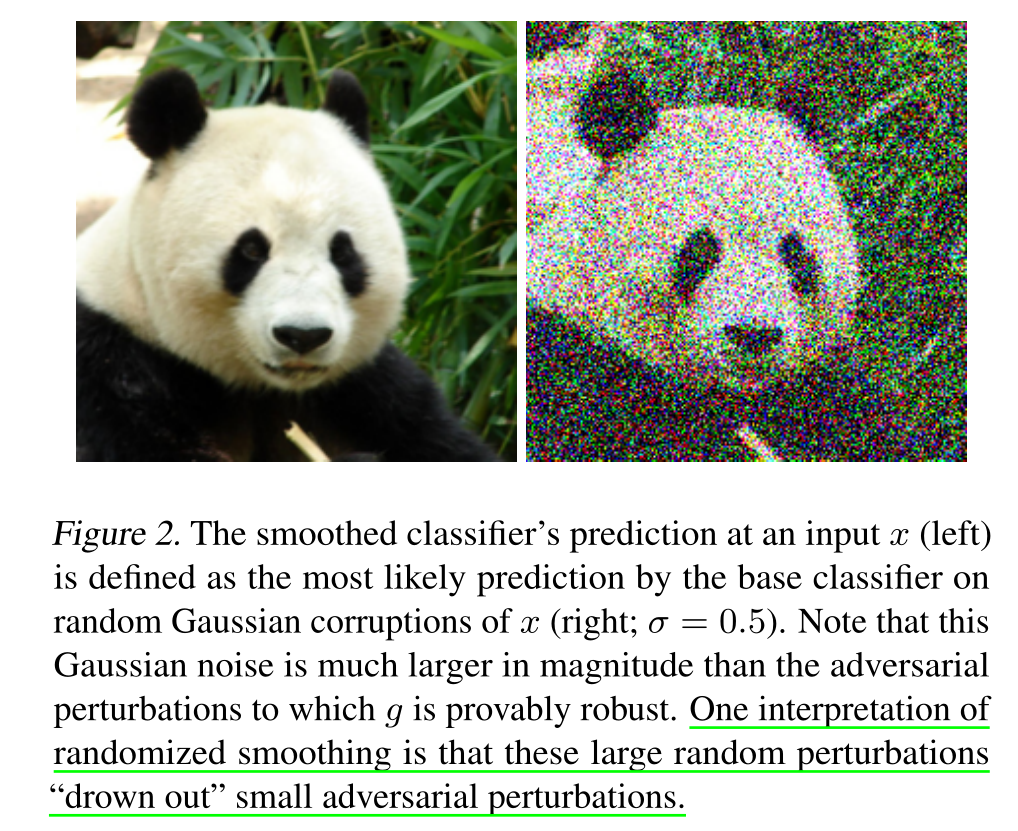
\includegraphics[width=0.4\linewidth]{1.png}
	\end{figure}
	One problem: How to measure the possibility? Sample
\end{frame}

\subsection{Robustness Guarantee}
\begin{frame}
	\frametitle{Robustness Guarantee}
	\begin{figure}
		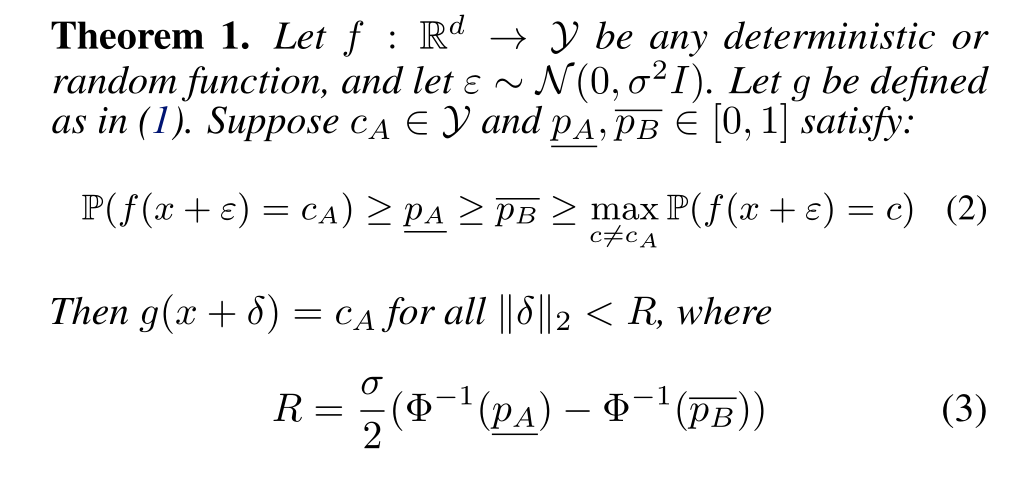
\includegraphics[width=0.4\linewidth]{2.png}
	\end{figure}
\end{frame}

\begin{frame}
	\frametitle{Illustration of the proof of Theorem 1}
	\begin{figure}
		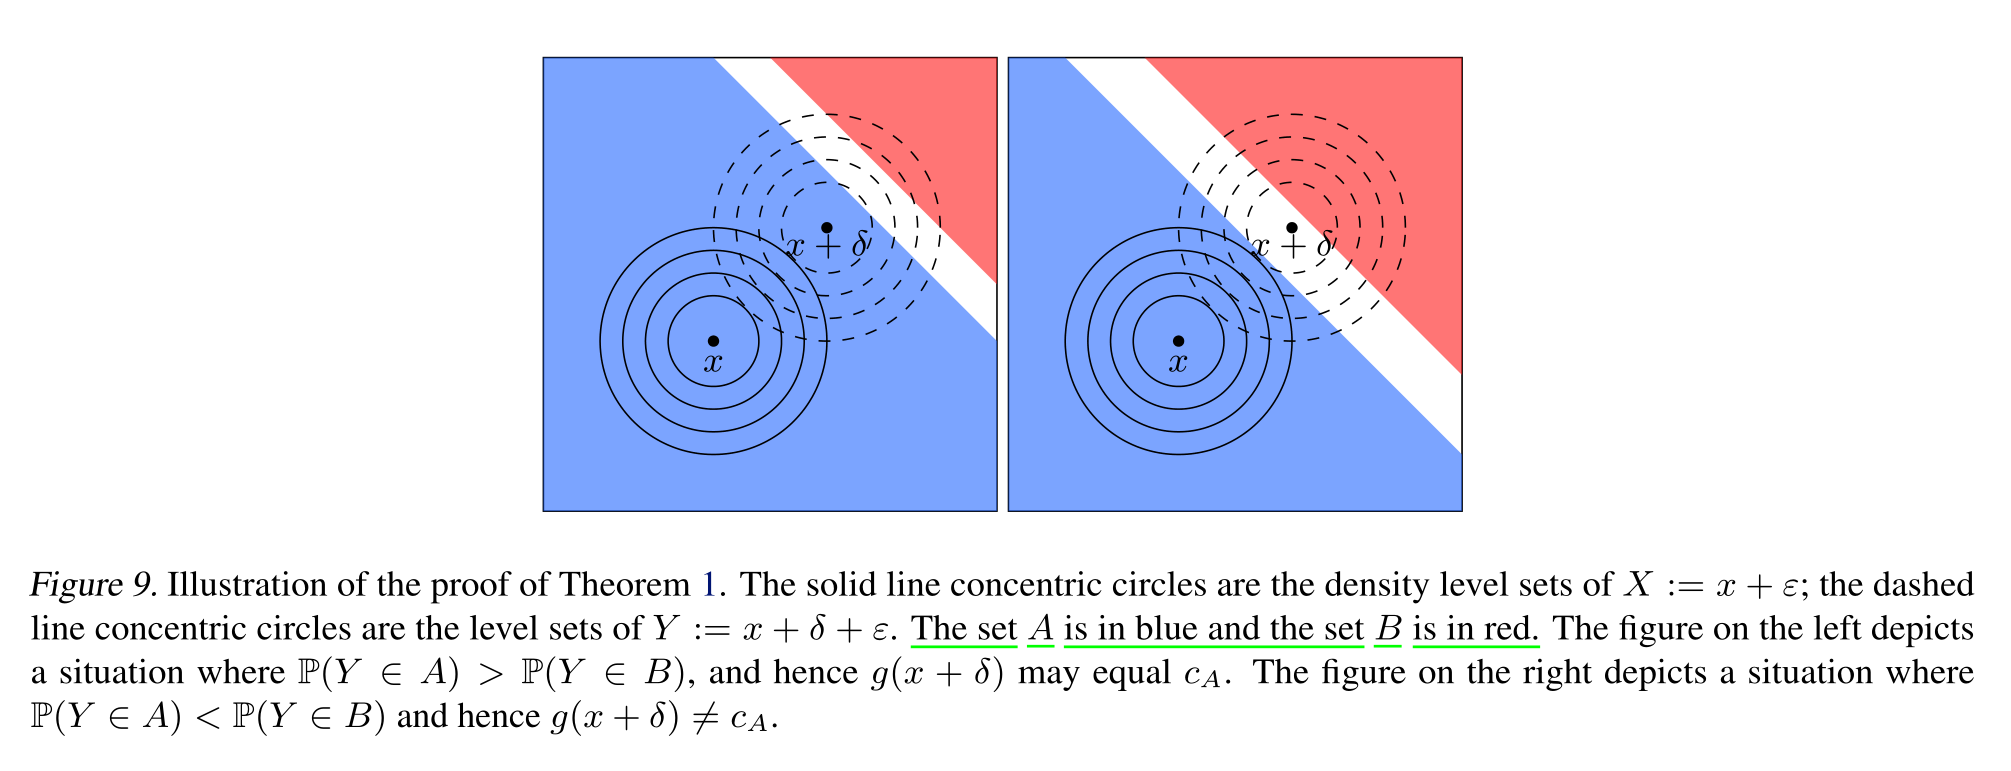
\includegraphics[width=0.9\linewidth]{3.png}
	\end{figure}
\end{frame}


\begin{frame}
	\frametitle{properties}
	\begin{itemize}
		\item Theorem 1 assumes nothing about $f$
		\item The certified radius $R$ is large when: (1) the noise level
		$\sigma$ is high, (2) the probability of the top class $c_A$ is high,
		and (3) the probability of each other class is low.
		\item The certified radius $R$ goes to $\infty$ as $p_{A} \rightarrow 1$ 
		and $\overline{p_{B}} \rightarrow 0 .$ This should sound reasonable: 
		the Gaussian distribution is supported on all of $\mathbb{R}^{d}$, so the only 
		way that $f(x+\varepsilon)=c_{A}$ with probability 1 is if $f=c_{A}$ almost everywhere.
	\end{itemize}
\end{frame}

\begin{frame}
	\frametitle{How, if $\delta > \| R \Vert$ } 
	\begin{figure}
		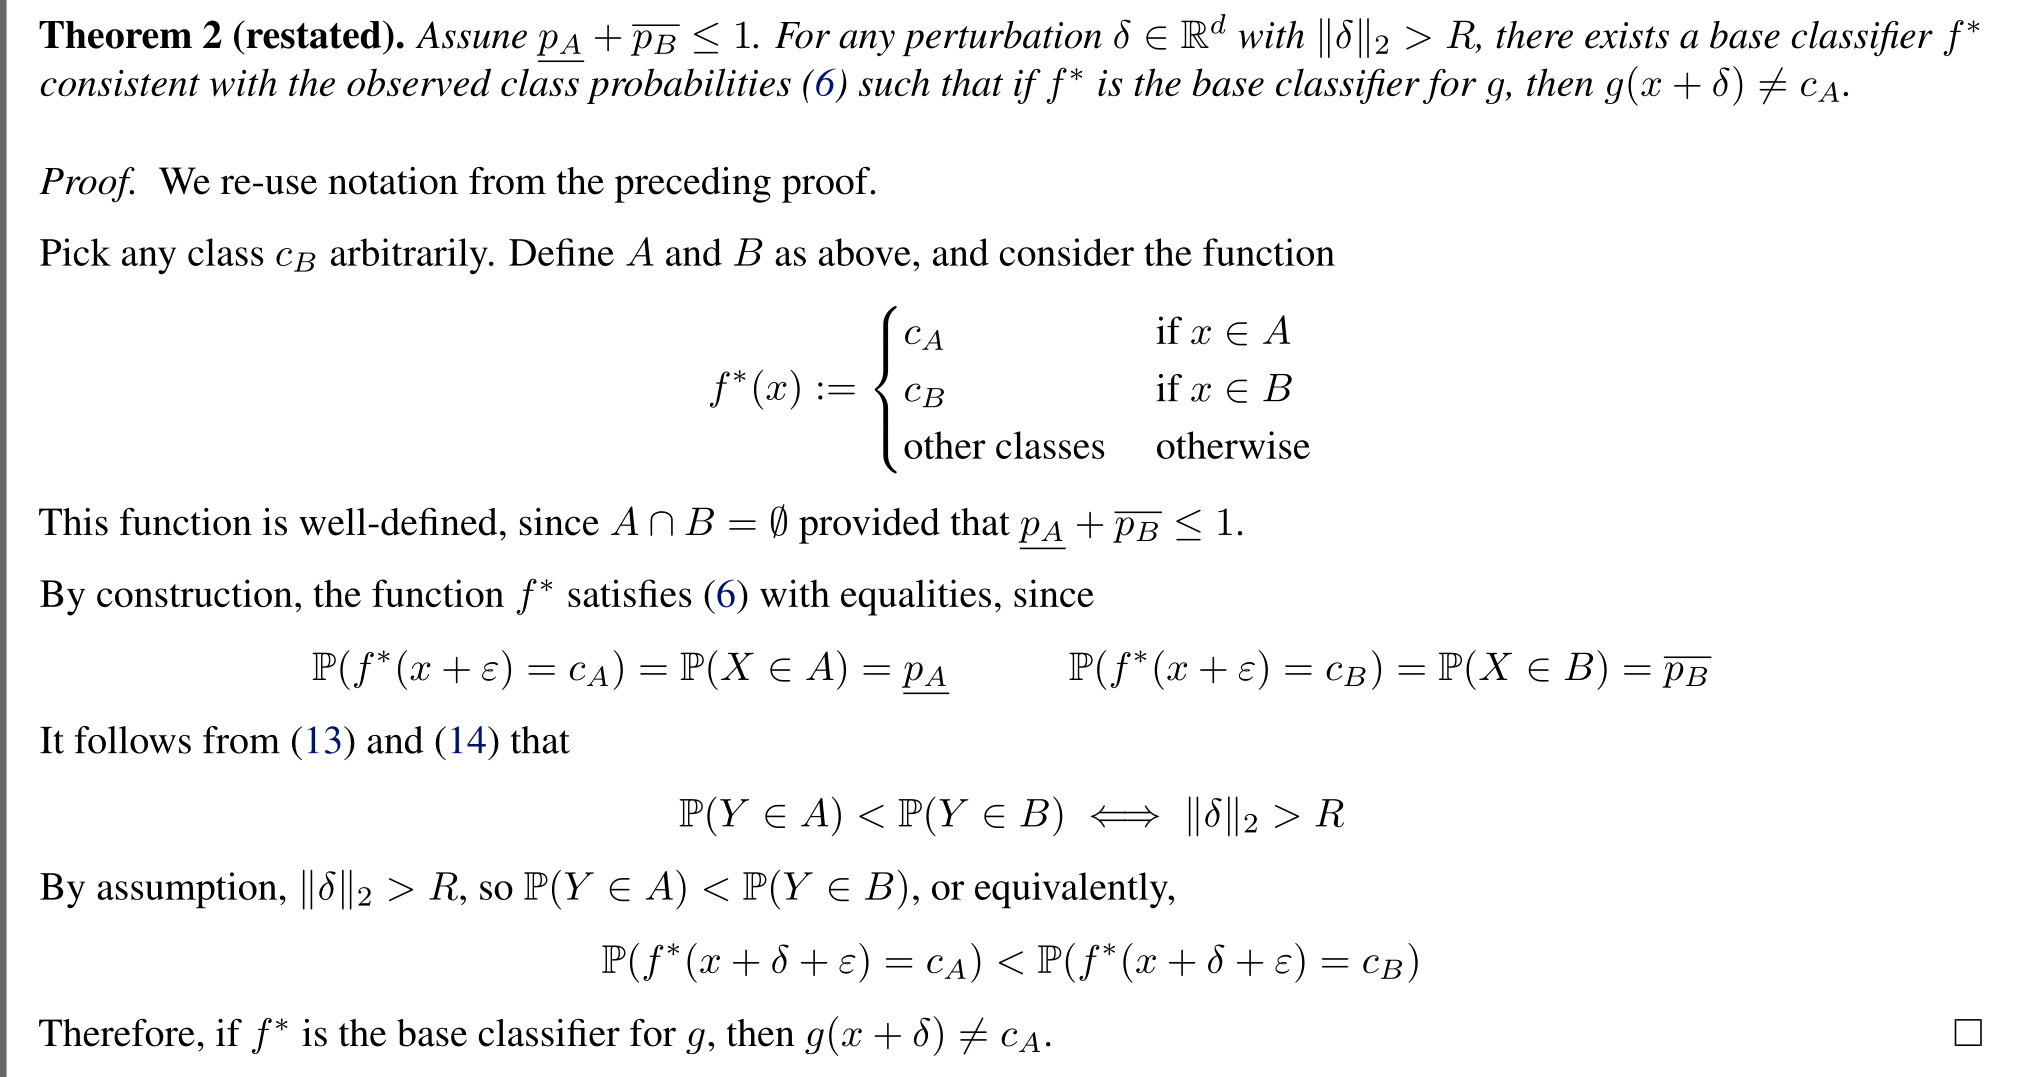
\includegraphics[width=0.8\linewidth]{6.png}
	\end{figure}
\end{frame}

\subsection{Special case}
\begin{frame}
	\frametitle{Binary Case}
	\begin{figure}
		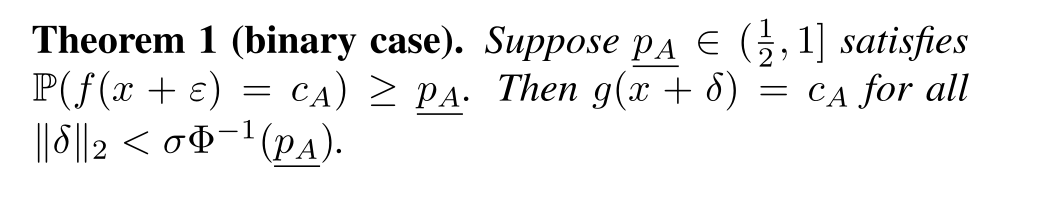
\includegraphics[width=0.8\linewidth]{7.png}
	\end{figure}
\end{frame}


\begin{frame}
	\frametitle{Linear base classifier}
	For two-class linear classifier
	$$
	f(x) = sign(w^Tx + b)
	$$

	we can get

	\begin{itemize}
		\item the distance from any input $x$ to the decision boundary is
		$$
		|w^Tx + b| / \Vert w \Vert ^2
		$$
		\item the smoothed classifier $g$ is identical to the base classifier $f$.
		\item  the true robust radius is $|w^Tx + b| / \Vert w \Vert$
	\end{itemize}
\end{frame}

\begin{frame}
	\frametitle{Noise level can scale with image resolution}
	\begin{figure}
		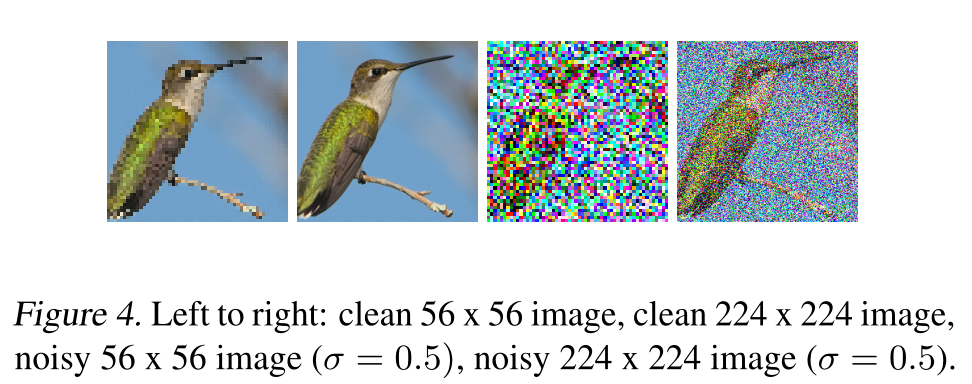
\includegraphics[width=0.8\linewidth]{8.png}
	\end{figure}
\end{frame}

\section{Practical algorithm}

\subsection{prediction}
\begin{frame}
	\frametitle{details}
	\begin{columns}
		\begin{column}{.4\textwidth}
			\begin{figure}[htbp]
				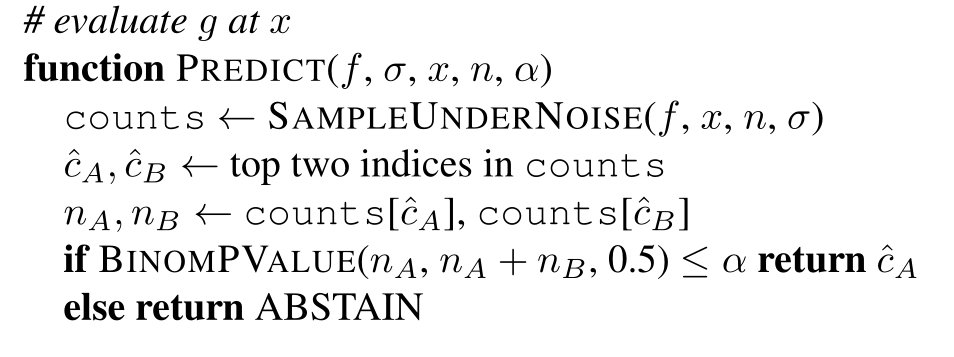
\includegraphics[width=1\linewidth]{10.png}
			\end{figure}
		\end{column}

		\begin{column}{.6\textwidth}
			\begin{figure}[htbp]
				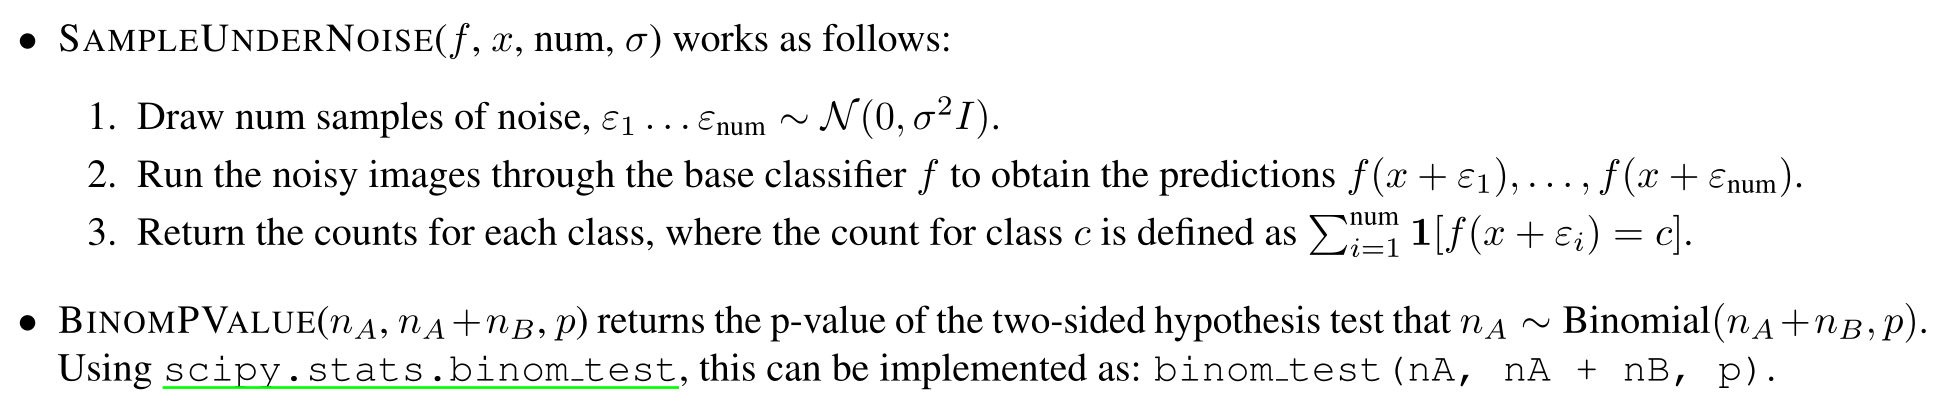
\includegraphics[width=1\linewidth]{11.png}
			\end{figure}
		\end{column}
	\end{columns}
	[1]Hung, K. and Fithian, W. Rank verification for exponential families. The Annals of Statistics, (2):758–782, 04 2019.
\end{frame}

\subsection{Certify}
\begin{frame}
	\frametitle{details}
	\begin{columns}
		\begin{column}{.4\textwidth}
			\begin{figure}[htbp]
				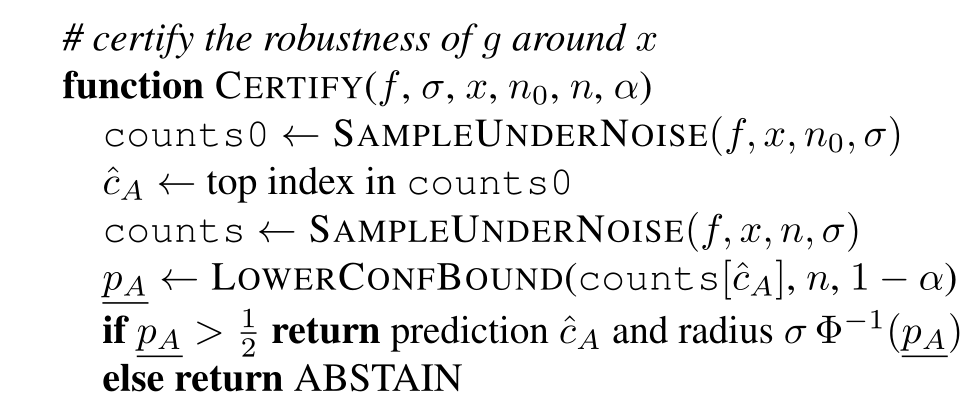
\includegraphics[width=1\linewidth]{12.png}
			\end{figure}
		\end{column}

		\begin{column}{.6\textwidth}
			\begin{figure}[htbp]
				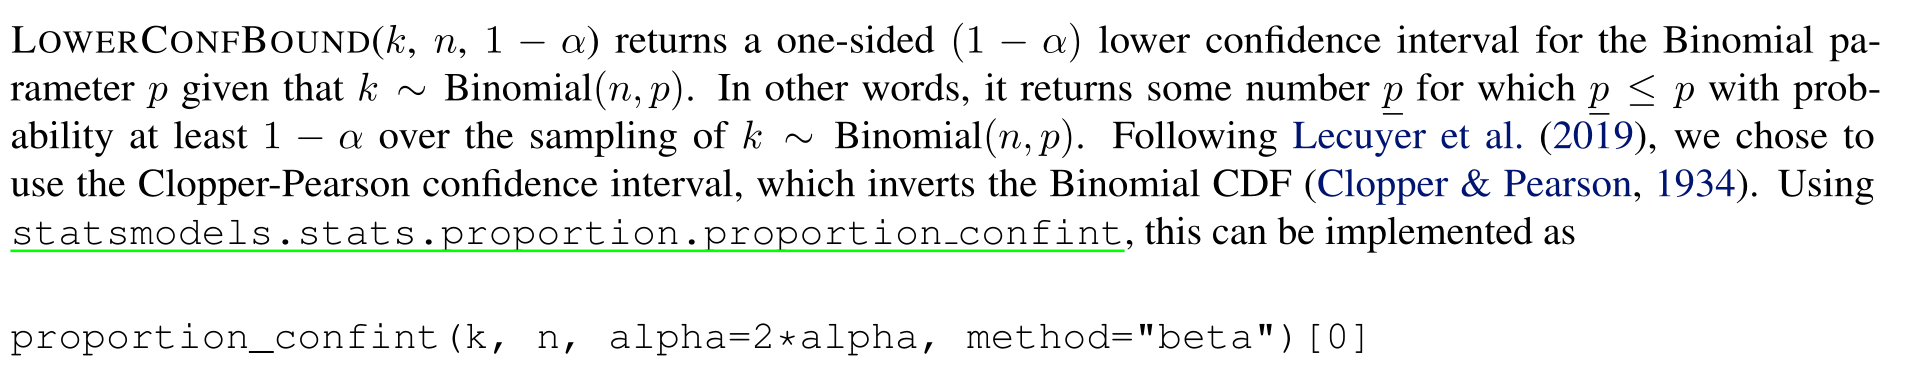
\includegraphics[width=1\linewidth]{13.png}
			\end{figure}
		\end{column}
	\end{columns}
	typical:the mass of $f(x+\varepsilon)$ not allocated to $c_A$ entirely to one runner-up class.
\end{frame}

\section{Experiment}
\subsection{Training}

\begin{frame}
	\frametitle{Gaussian data augmentation}
	\begin{itemize}
		\item In order for $g$ to classify the labeled example $(x, c)$ 
		correctly and robustly, f needs to consistently classify $\mathcal{N}(x, \sigma^2I)$ as $c$
		\item In high dimension, the Gaussian distribution 
		$\mathcal{N}(x, \sigma^2I)$ places almost no mass near 
		its mode x. 
		\item As a consequence, when σ is moderately high, the distribution 
		of natural images has virtually disjoint support from the 
		distribution of natural images corrupted by $\mathcal{N}(x, \sigma^2I)$
		\item Therefore, if the base classifier $f$ is trained via 
		standard supervised learning on the data distribution, 
		it will see no noisy images during training
	\end{itemize}
	
\end{frame}

\subsection{result}
\begin{frame}
	\frametitle{mnist\&ImageNet}
	\begin{columns}
		\begin{column}{.4\textwidth}
			\begin{figure}[htbp]
				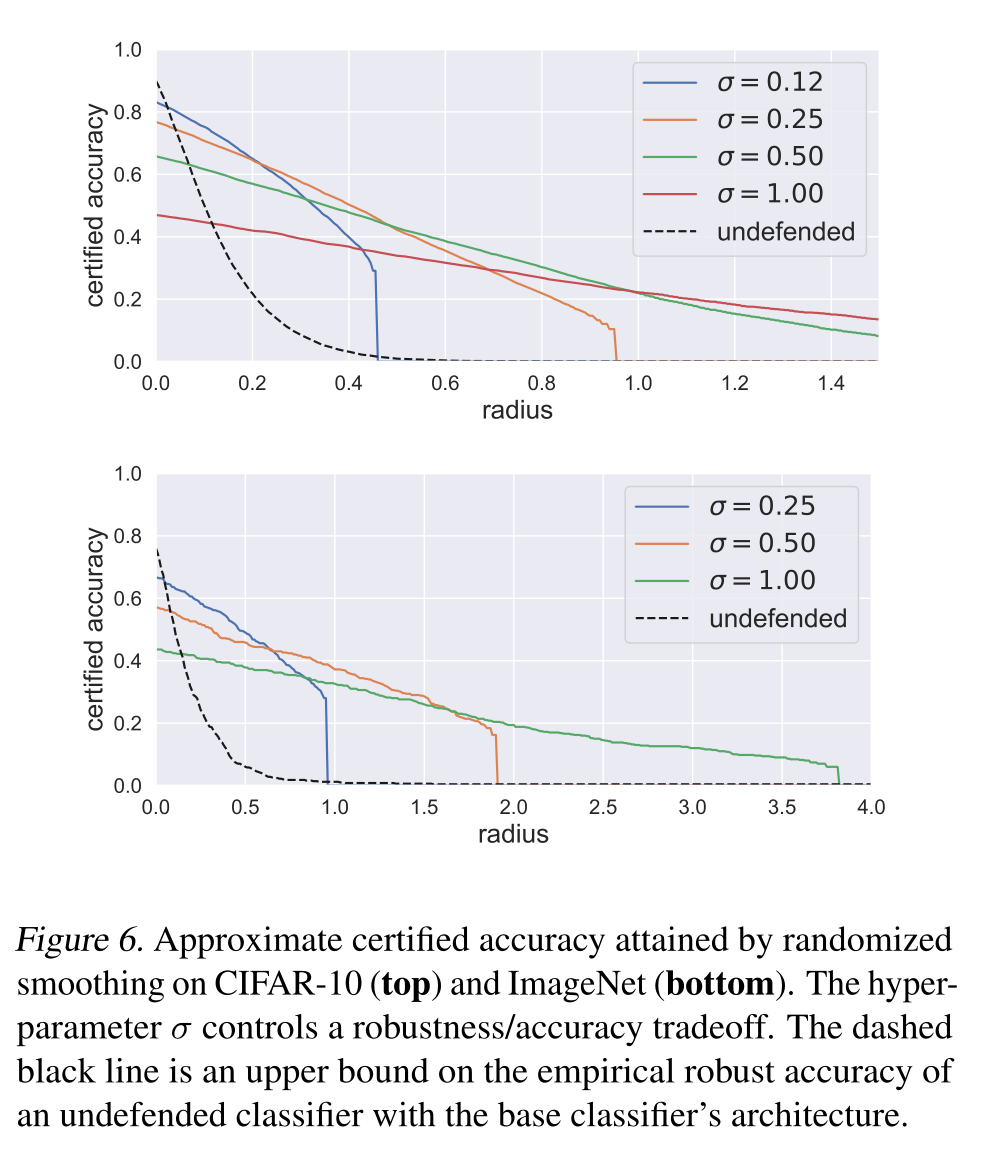
\includegraphics[width=.8\linewidth]{16.png}
			\end{figure}
		\end{column}

		\begin{column}{.6\textwidth}
			\begin{itemize}
				\item $\alpha = 0.001,n_0 = 100, n = 10^5$
				\item there is a hard upper limit to the radius
				\item CIFAR-10 :110-layer residual network; certifying each example took 15 seconds on an NVIDIA RTX 2080 Ti. 
				\item ImageNet :base classifier - ResNet-50; took 110 seconds.
				\item Full CIFAR-10 test set and 500 examples from the ImageNet test set.
				\item Black line:DeepFool $l_2$ adversarial attack
				\item Blance between accuracy and radii 
			\end{itemize}
		\end{column}
	\end{columns}	
\end{frame}

\begin{frame}
	\frametitle{Result}
	\begin{figure}[htbp]
		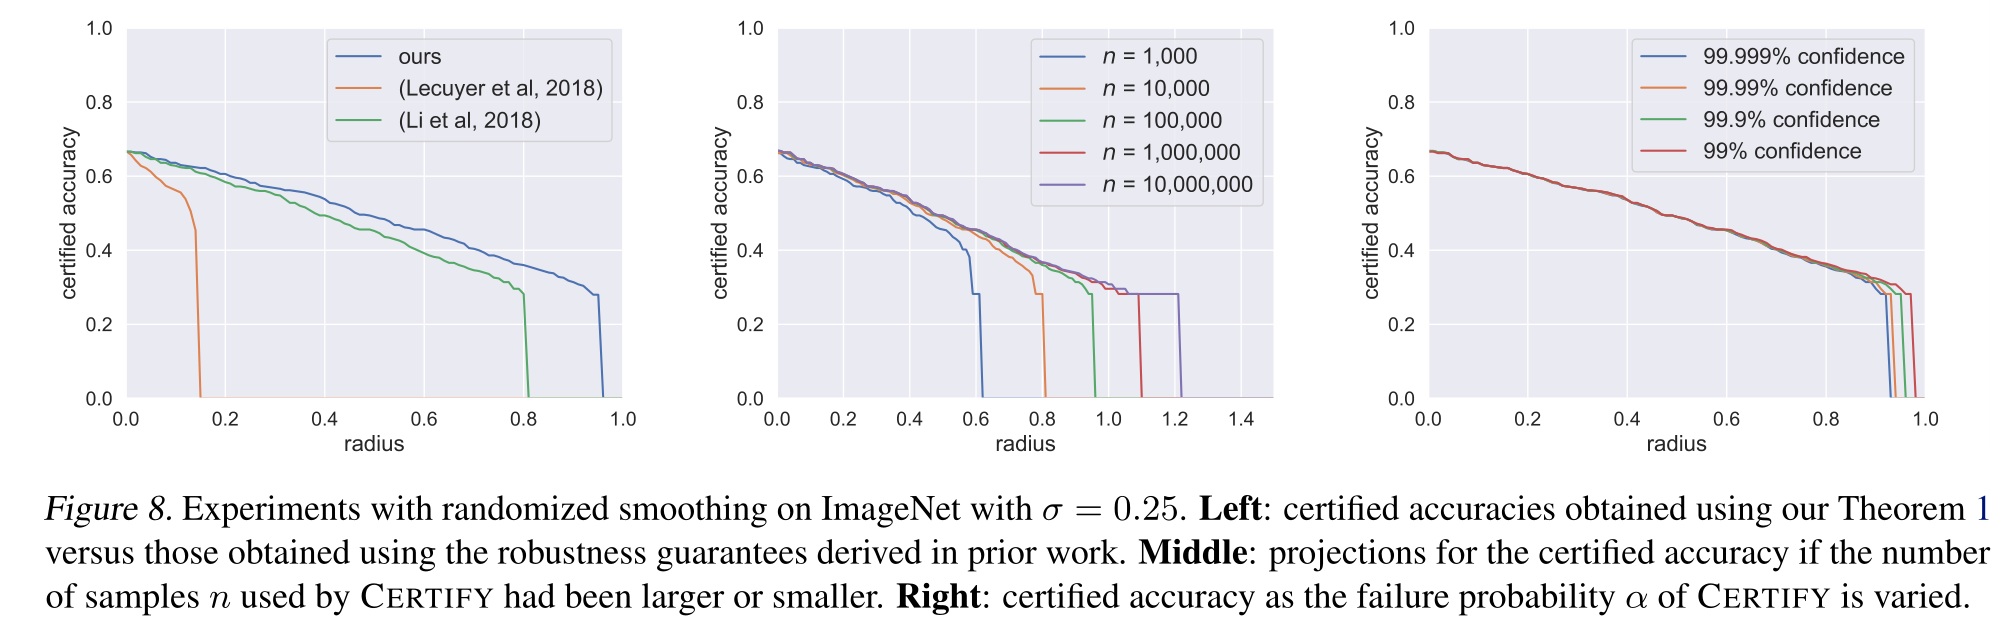
\includegraphics[width=1\linewidth]{17.png}
	\end{figure}
\end{frame}


\begin{frame}
	\frametitle{Comparison to baselines}
	\begin{figure}[htbp]
		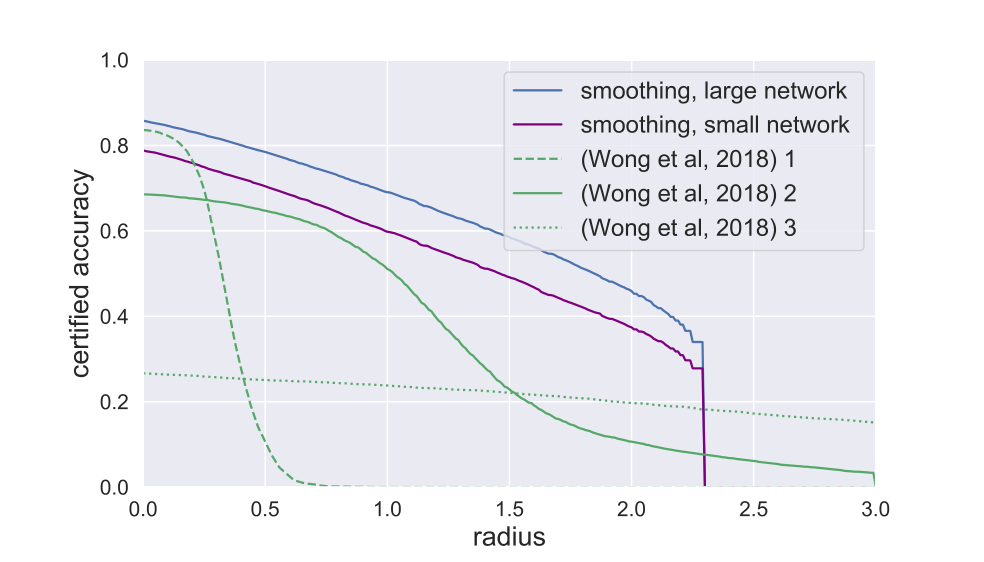
\includegraphics[width=.5\linewidth]{18.png}
	\end{figure}

	\begin{itemize}
		\item [2]Wong, E., Schmidt, F., Metzen, J. H., and Kolter, J. Z. Scaling provable 
		adversarial defenses. In Advances in Neural Information Processing Systems 31, 2018
	\end{itemize}
	

\end{frame}

\begin{frame}
	\frametitle{Prediction}
	\begin{figure}[htbp]
		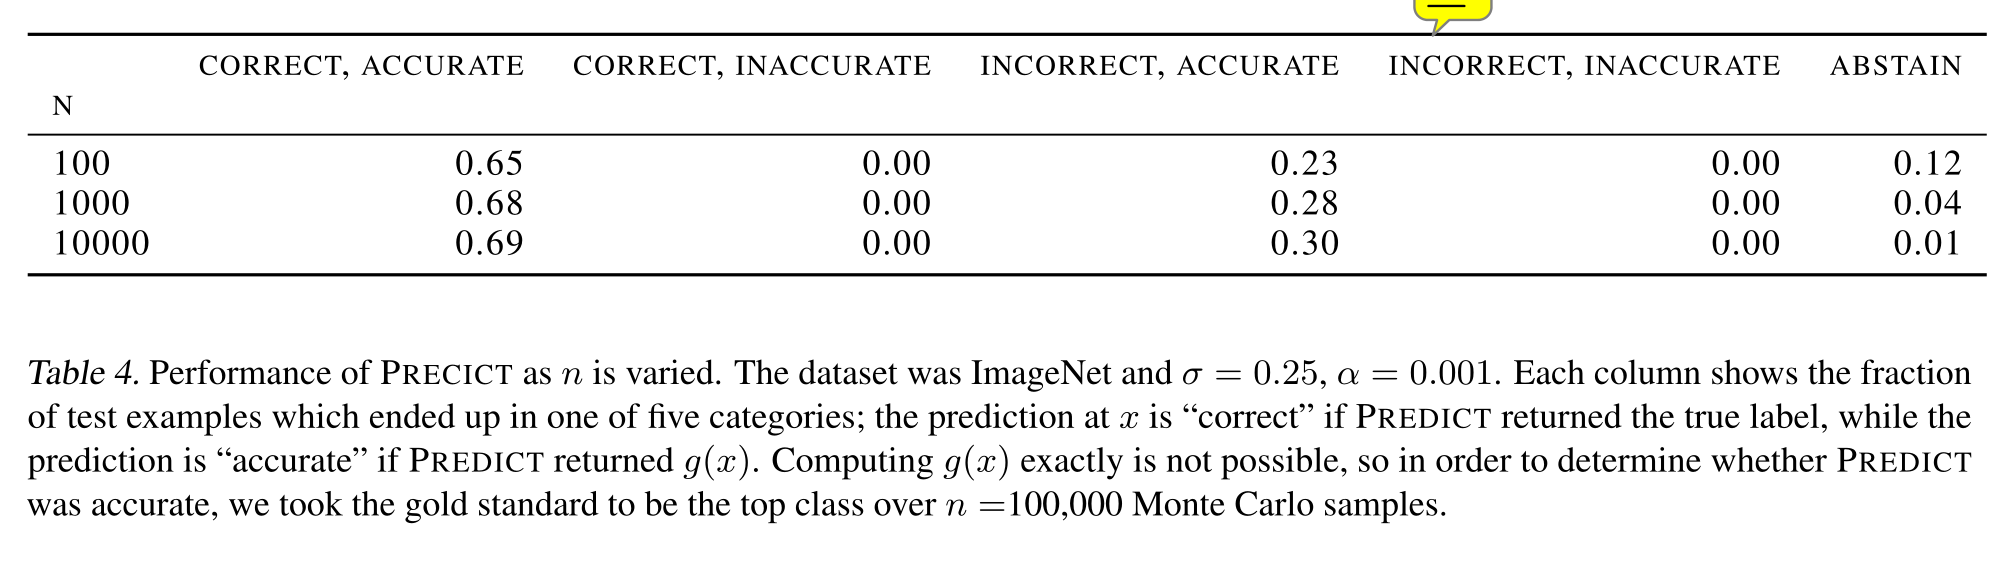
\includegraphics[width=1\linewidth]{19.png}
	\end{figure}
\end{frame}

\begin{frame}
	\frametitle{Attack}
	\begin{itemize}
		%\item When $f$ is linear, there always exists a class-changing perturbation just beyond the
		%certified radius.
		\item PGD:empirically assess the tightness of our bound 
		\item If the example was correctly classified and certified robust at radius $R$, 
		we tried finding an adversarial example for $g$ within radius $1.5R$ and 
		within radius $2R$. We succeeded 17\% of the time at radius $1.5R$ and 53\% 
		of the time at radius $2R$.
	\end{itemize}	
\end{frame}



%------------------------------------------------


%------------------------------------------------

%------------------------------------------------


%------------------------------------------------
\begin{frame}
\hfill
\center{\Huge{\calligra{\Huge{Thank you}}}}
\linespread{3}\selectfont
\end{frame}
%----------------------------------------------------------------------------------------
\end{document}